\documentclass[a4paper,12pt]{article}
\usepackage{listings}  %cpp code
\usepackage[T1,T2A]{fontenc}
\usepackage[utf8]{inputenc}
%\renewcommand{\rmdefault}{ftm}-TimesNewRoman
\usepackage[14pt]{extsizes}
\usepackage[ukrainian]{babel}
\usepackage{amsmath}
\usepackage{tikz}
\usepackage{pgfplots}
\usepackage{gnuplottex}
\usepackage{graphicx}
\usepackage{gensymb}
\usepackage{graphicx}
\usepackage{subcaption}
\graphicspath{{pictures/}}
\DeclareGraphicsExtensions{.pdf,.png,.jpg,.gif}
\pgfplotsset{compat = 1.3}
\sloppy %-rastiazhenie abzaca
\relpenalty=10000
\pagestyle{plain}
\begin{document}
\title{\HugeЗвіт до лабораторної роботи №3\linebreak }
\author{\LargeВиконали: Дирів Олександр та Рябоконь Максим}
\date{}
\maketitle
\newpage
{\Large\tableofcontents}
\newpage
\section{Мигання світлодіодом}
\quad У цьому пункті були отримані блимання світлодіода за допомогою плати Arduino Uno. Для цього було зібрано схему, зображену на Рис. 1. Світлодіод був підключений послідовно з резистором, який обмежує струм. Опір резистора 330 Ом, краще б взяти менший, але такого не було в наявності тому діод не максимально яскравий.
\par\quad\begin{figure}[!h]
  \centering
 \begin{subfigure}[b]{0.6\linewidth}
    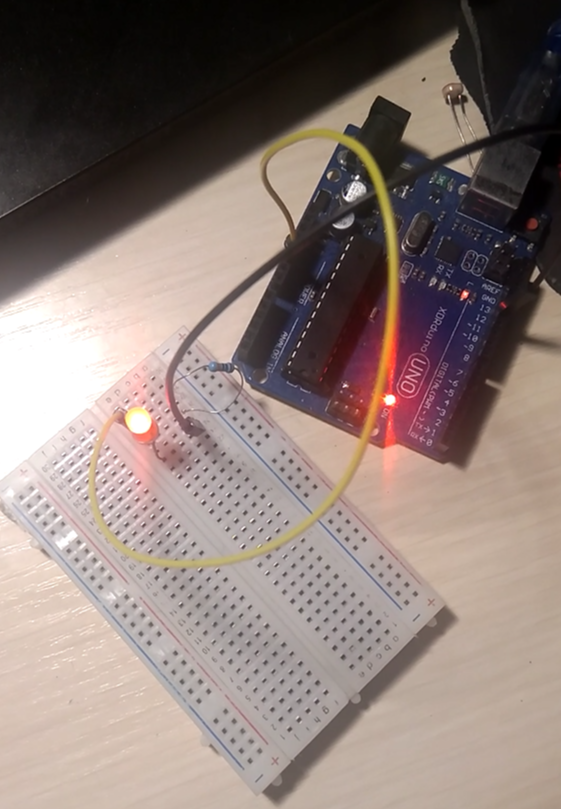
\includegraphics[width=\linewidth]{diode.PNG}
  \end{subfigure}
  \caption{}
\end{figure}
\par\quad\begin{figure}[!h]
  \centering
 \begin{subfigure}[b]{1\linewidth}
    \includegraphics[width=\linewidth]{di.png}
  \end{subfigure}
  \caption{}
\end{figure}
\clearpage
\section{Потенціометр}
\quad У цьому пункті, оскільки в наявності не було світлодіодного індикатора, зібрана схема управління яскравістю світлодіода за допомогою потенціометра(див Рис. 3). Простий приклад використання аналогового входу та виходу плати.
\par\quad\begin{figure}[!h]
  \centering
 \begin{subfigure}[b]{0.6\linewidth}
    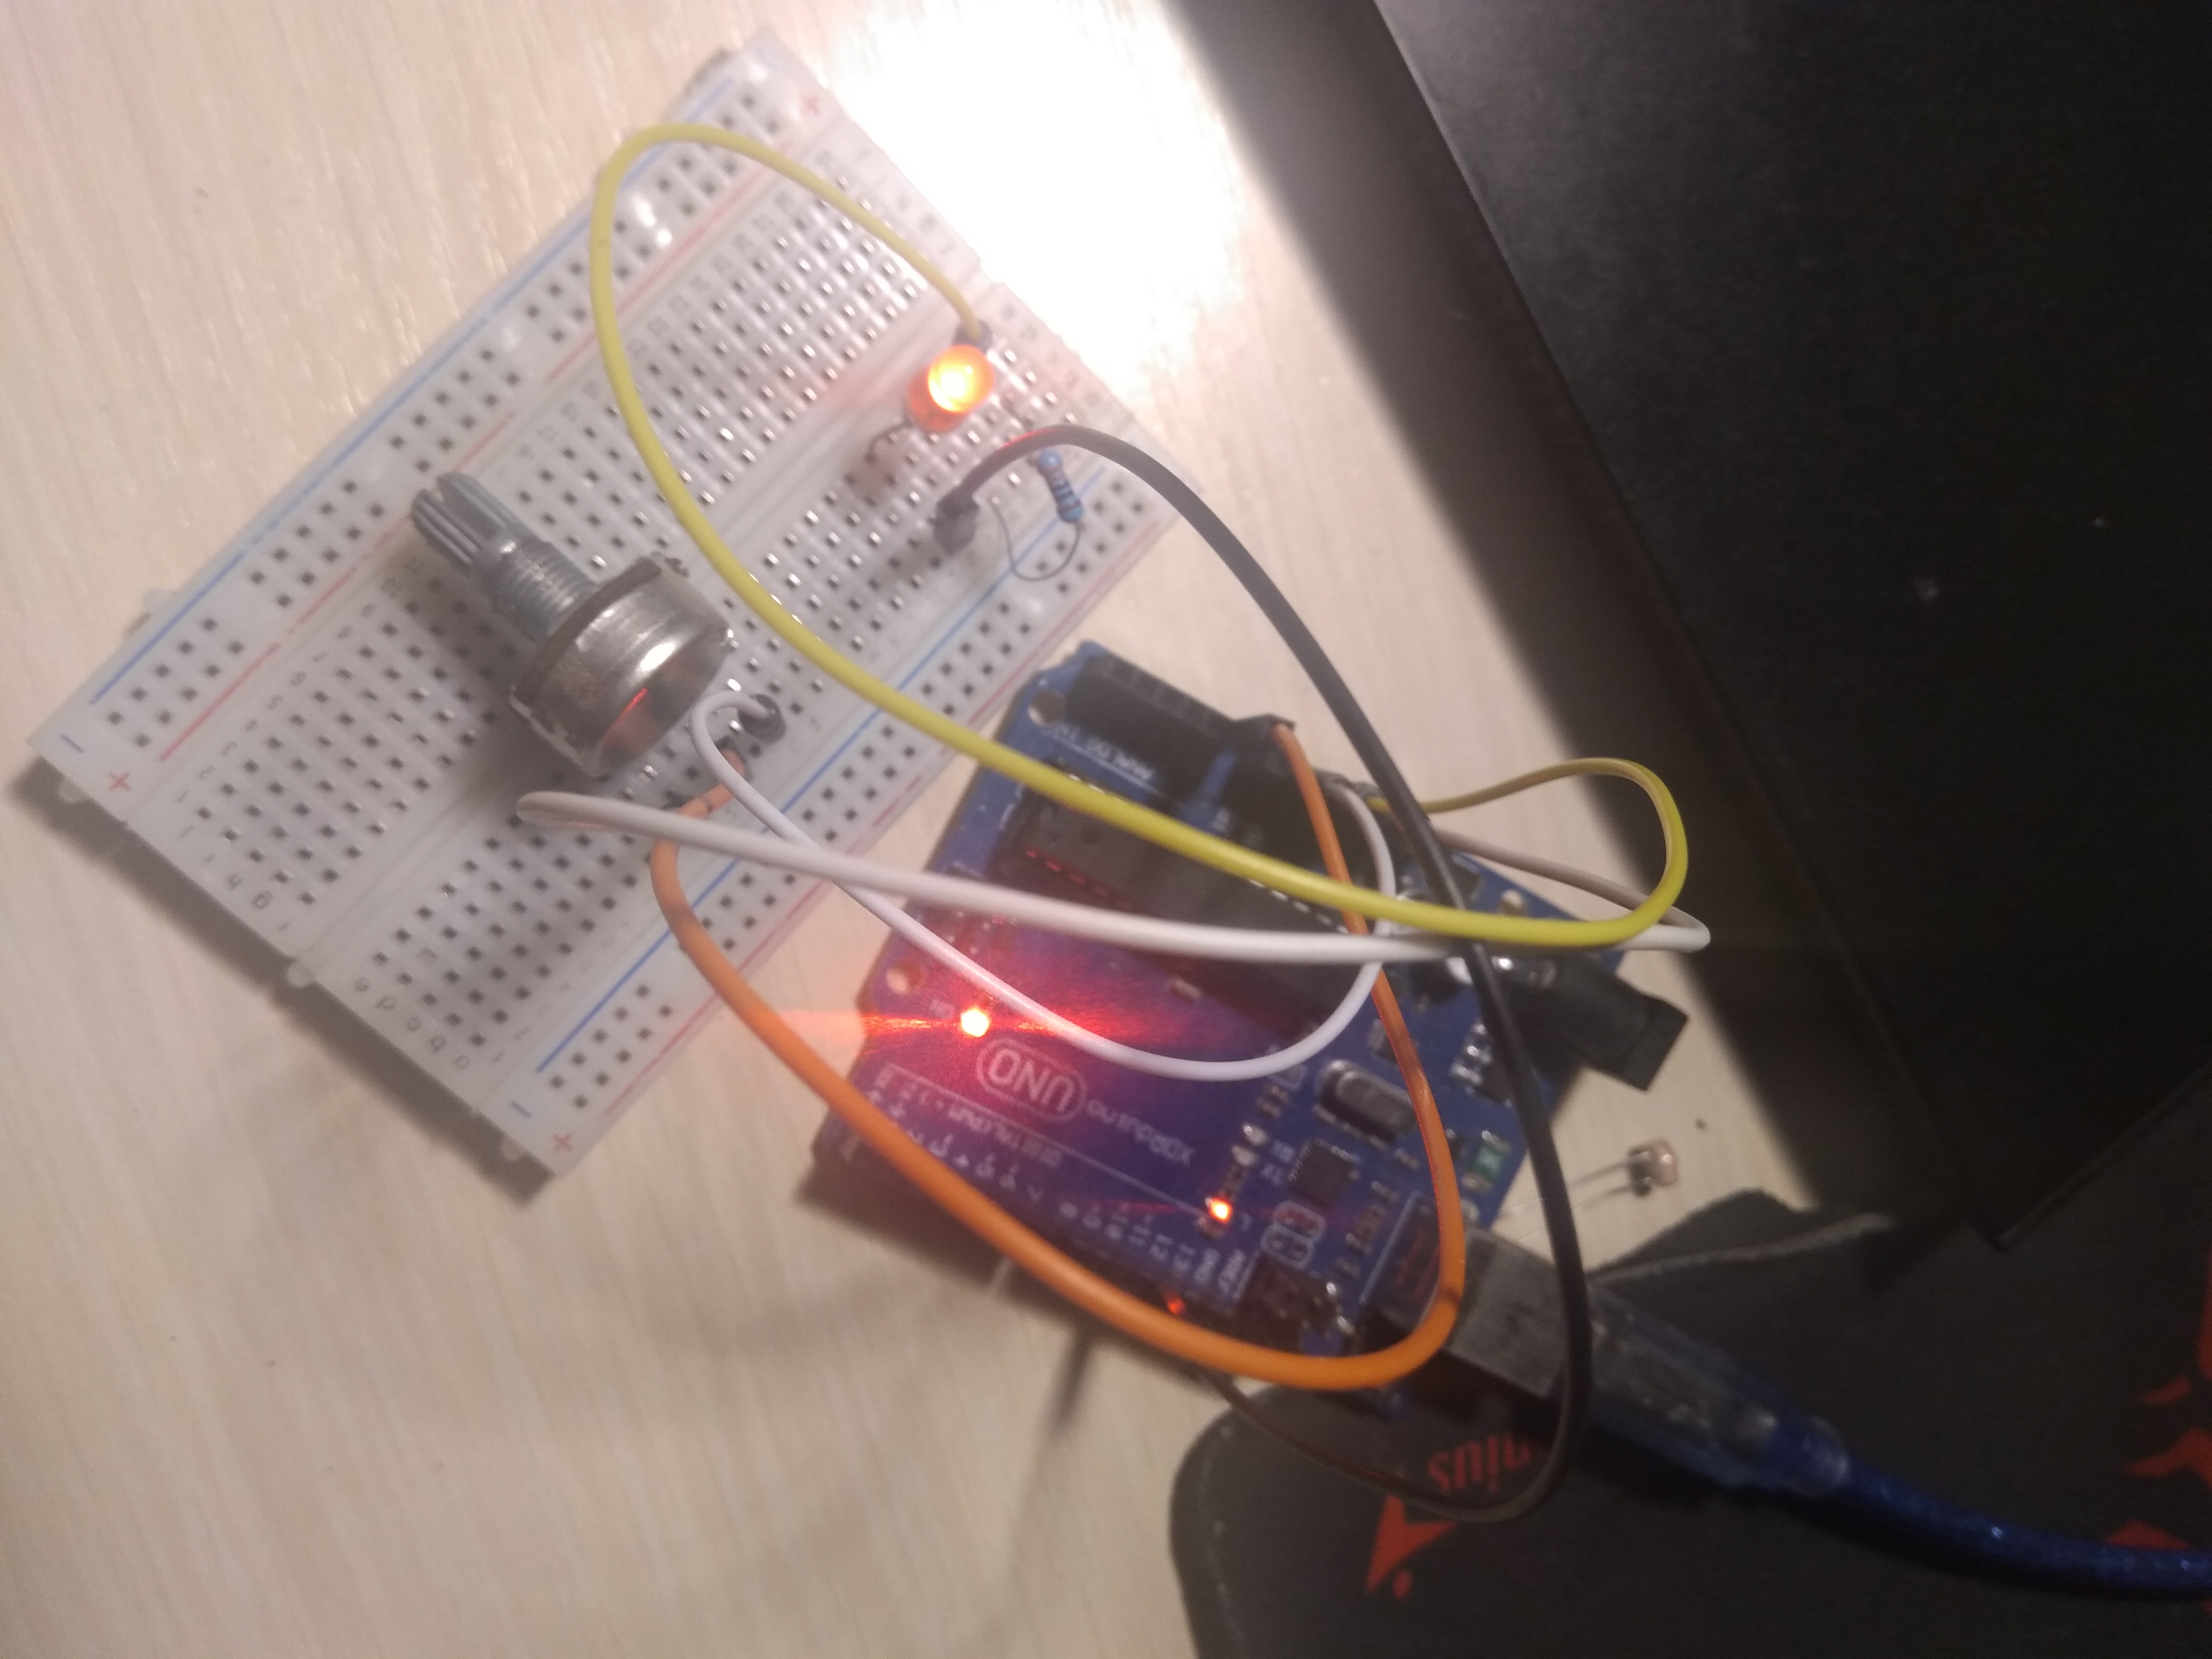
\includegraphics[width=\linewidth]{potentiometer.jpg}
  \end{subfigure}
  \caption{}
\end{figure}
\par\quad\begin{figure}[!h]
  \centering
 \begin{subfigure}[b]{1\linewidth}
    \includegraphics[width=\linewidth]{pot.png}
  \end{subfigure}
  \caption{}
\end{figure}
\clearpage
\section{Виведення освітлення за допомогою фоторезистора}
\par У даному пункті було виведено освітленість на два світлодіоди, оскільки в наявності було лише 6 дротів. Освітленість вимірювалась за допомогою фоторезистора. Для цього фоторезистор був підключений послідовно до резистора, утворюючи подільник напруги. Середня точка між ними підключена до ніжки A3 Arduino, напруга там постійно вимірюється за допомогою аналого-цифрового перетворювача, вбудованого в Arduino. Також я випадково вимірював напругу на резисторі тому аналогові значення не досягають максимуму а також при збільшенні освітленості збільшуються, оскільки опір фоторезистора зменшується.
\par\quad\begin{figure}[!h]
  \centering
 \begin{subfigure}[b]{0.6\linewidth}
    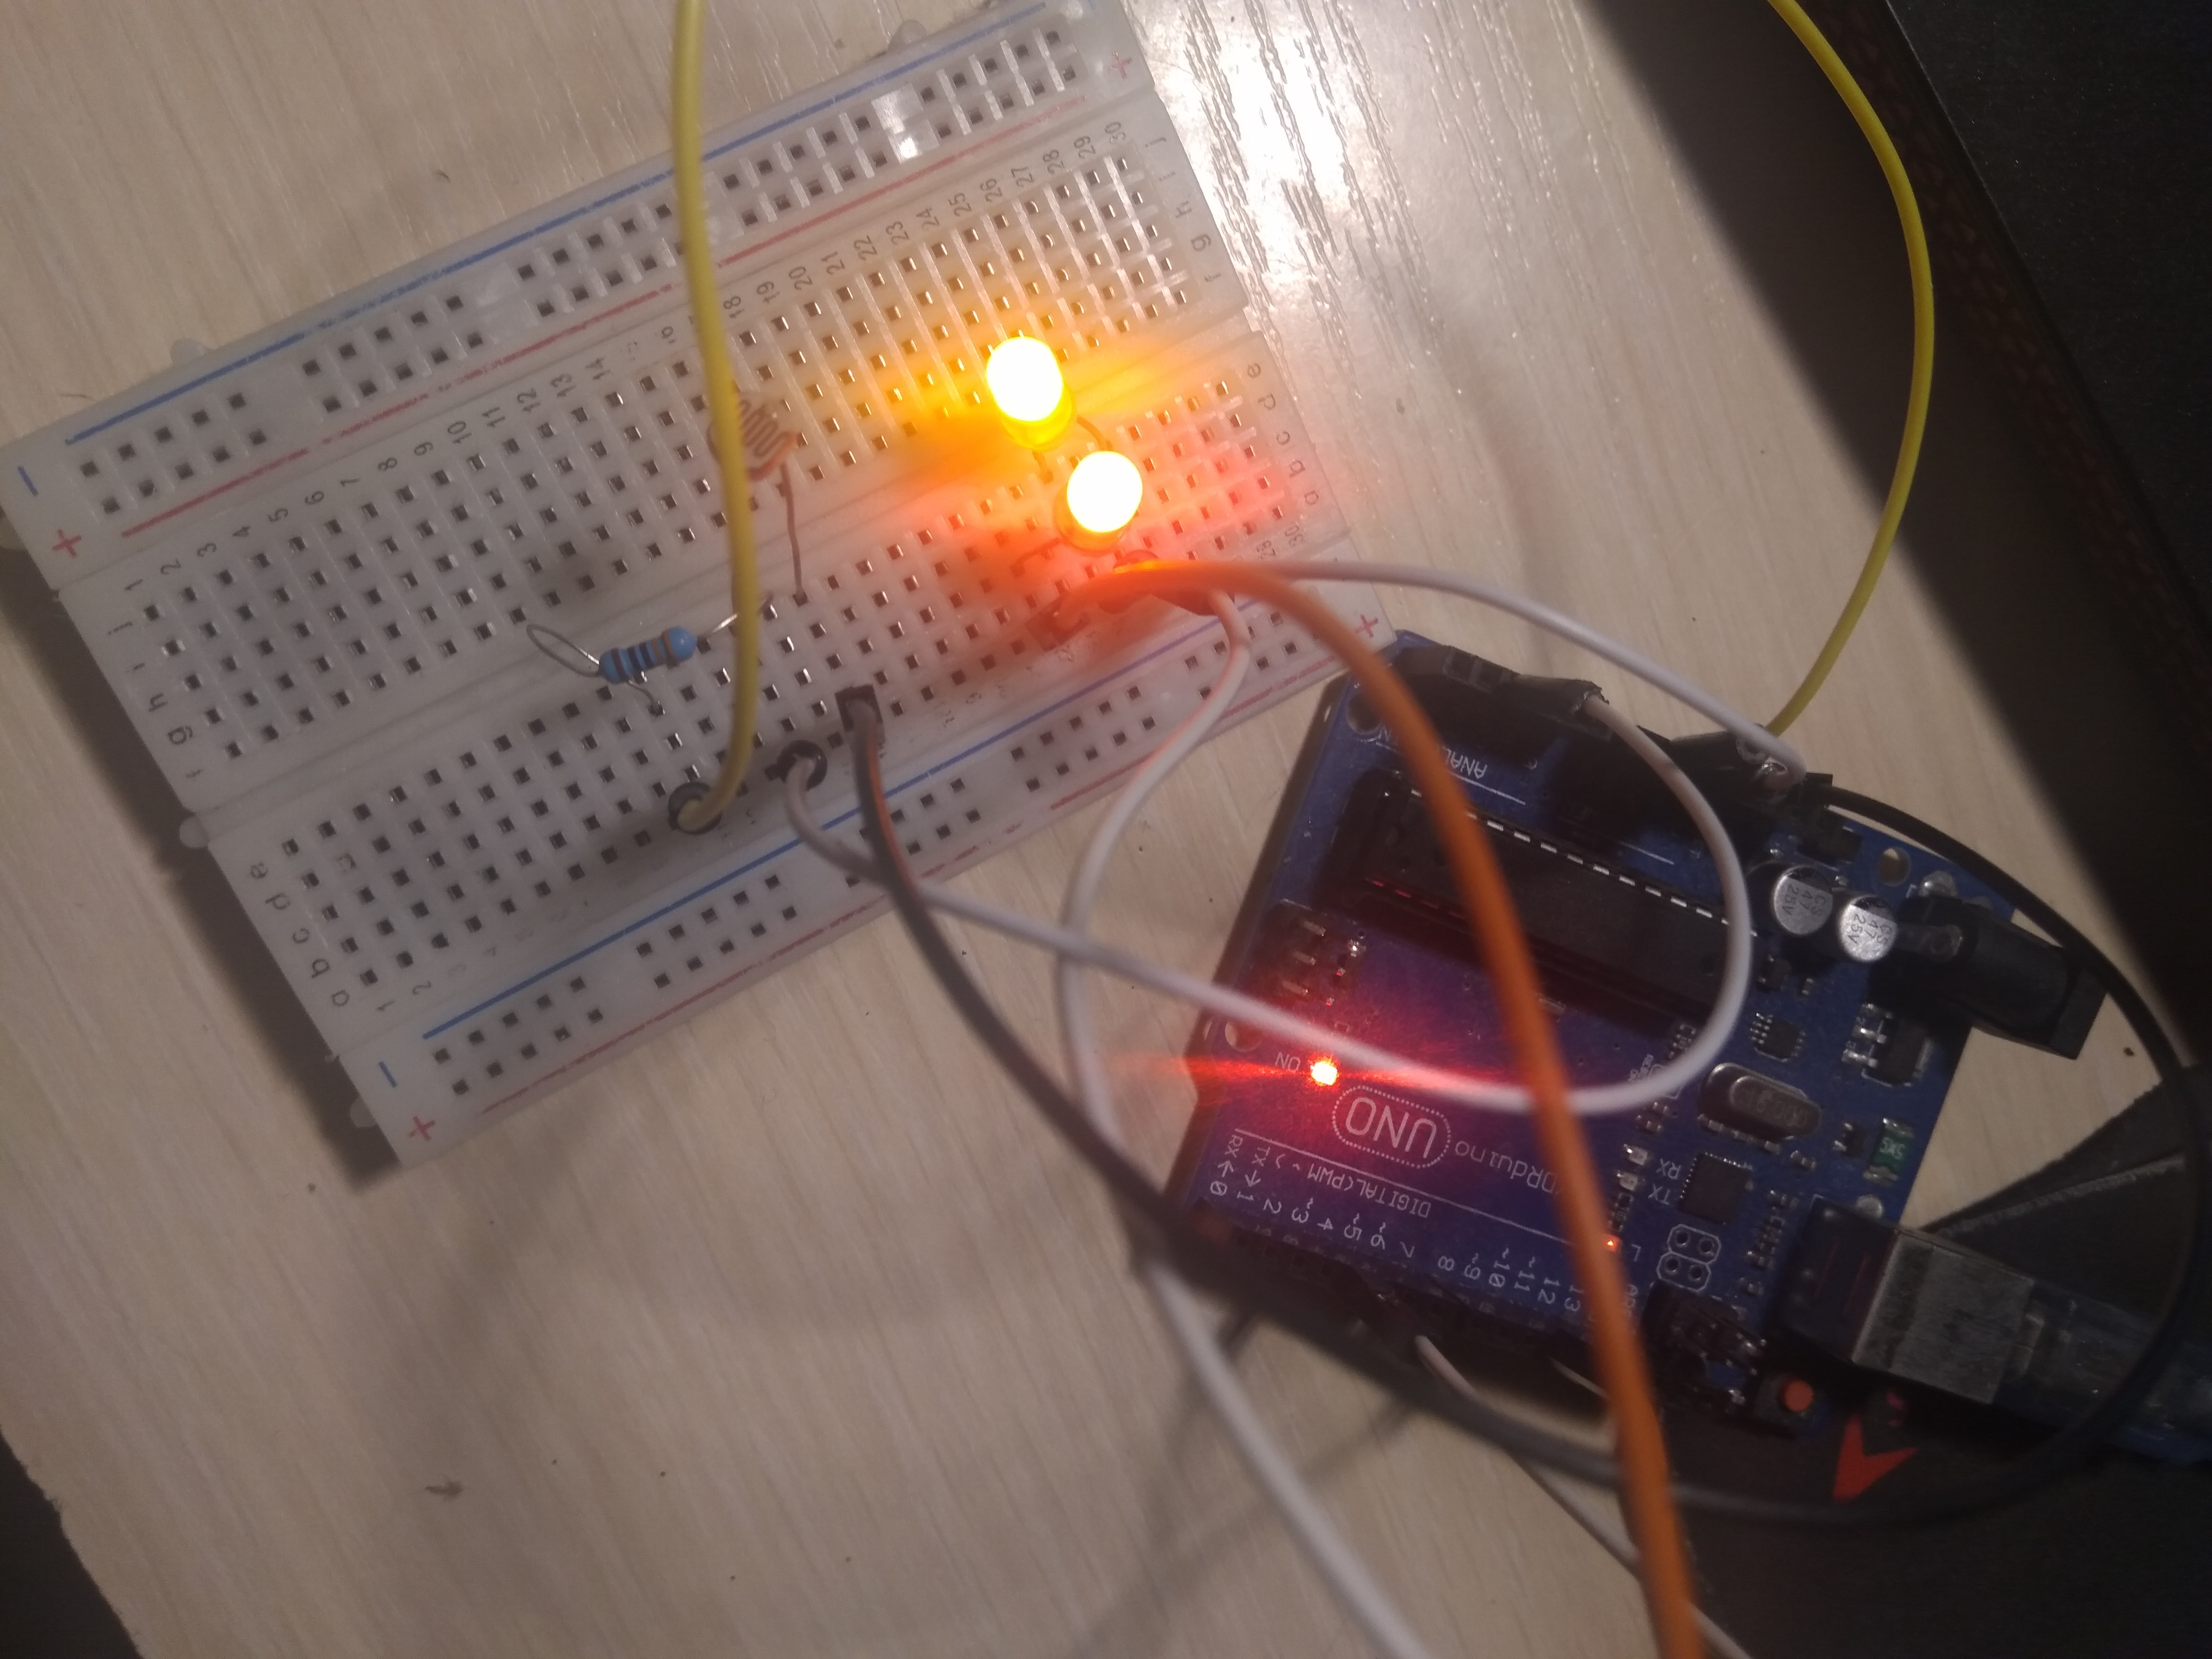
\includegraphics[width=\linewidth]{photoresistor.jpg}
  \end{subfigure}
  \caption{}
\end{figure}
\par\quad\begin{figure}[!h]
  \centering
 \begin{subfigure}[b]{1\linewidth}
    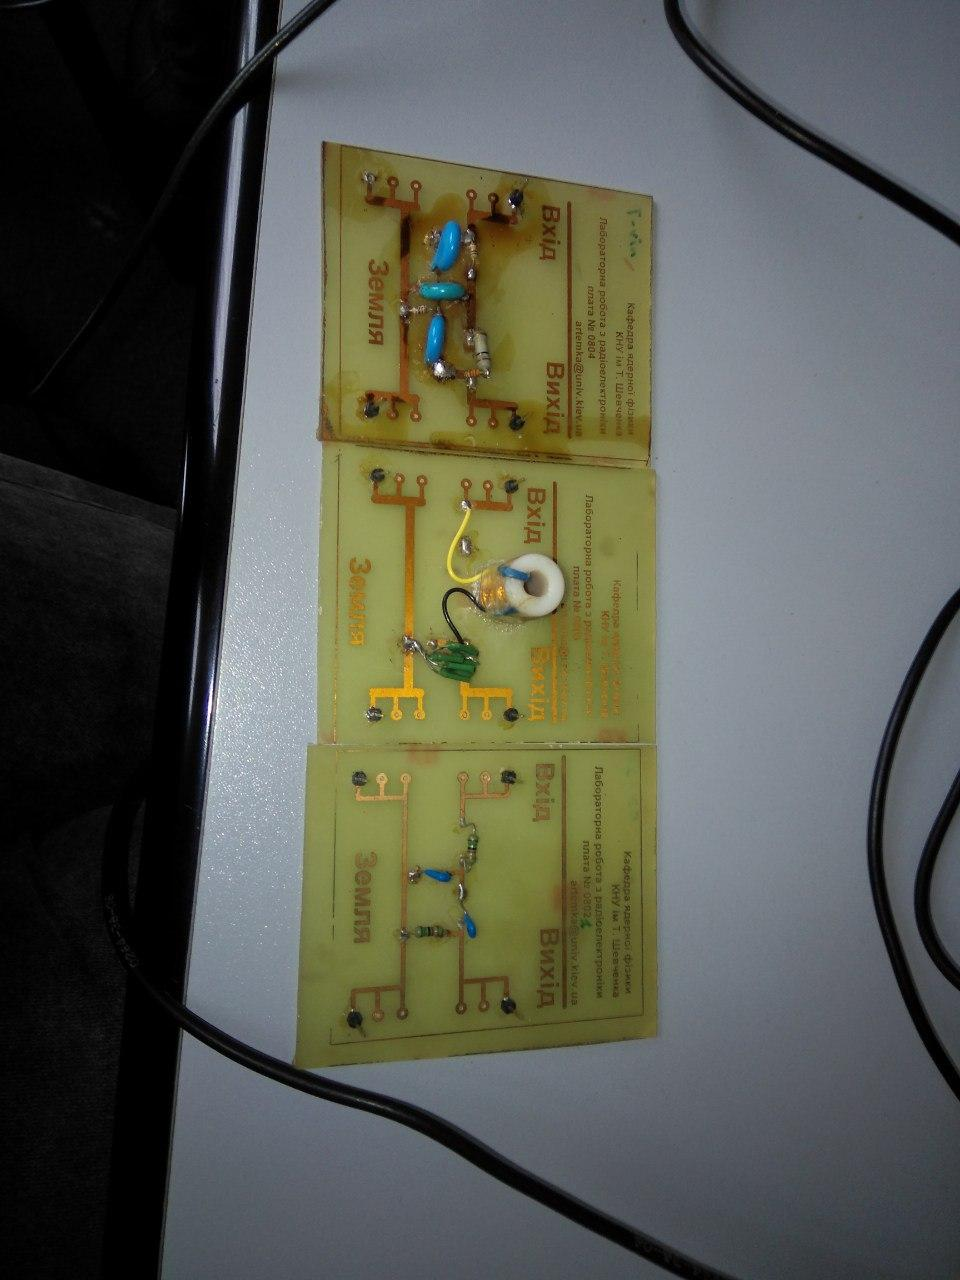
\includegraphics[width=\linewidth]{photo.png}
  \end{subfigure}
  \caption{}
\end{figure}

\clearpage\section{Висновки}
\par\quadУ результаті даної лабораторної роботи були реалізовані такі задачі:
\par\quad1) Мигання світлодіода
\par\quad2) Світлодіод, яскравість якого контролює потенціометр
\par\quad3) Виведення освітлення за допомогою фоторезистора
\end{document}